% questions.tex —— 2025 年·全国 1 卷 · 题目内容片段（无答案）
% 由 tools/generate_projects.py 依来源总账自 2025/2025_数学真题_试题.md 生成，勿手改（改源 MD 后重跑）


\begin{gknotice}
\textbf{适用省份}：山东、广东、湖南、湖北、河北、江苏、福建、浙江、河南、江西、安徽
\end{gknotice}

\par\medskip

\gkpart{一、单选题}

\begin{gktip}
本题共 8 小题，每小题 5 分，共 40 分。在每小题给出的四个选项中，只有一项是符合题目要求的。
\end{gktip}

\begin{question}
\gkti{1}$(1+5\mathrm{i})\mathrm{i}$ 的虚部为（　　）

\begin{gkopts}(4)
\task A．$-1$
\task B．$0$
\task C．$1$
\task D．$6$
\end{gkopts}

\end{question}
\begin{question}
\gkti{2}已知集合 $U=\{x\mid x\text{ \text{是小于} }9\text{ \text{的正整数}}\}$，$A=\{1,3,5\}$，则 $\complement_U A$ 中元素的个数为（　　）

\begin{gkopts}(4)
\task A．$0$
\task B．$3$
\task C．$5$
\task D．$8$
\end{gkopts}

\end{question}
\begin{question}
\gkti{3}已知双曲线 $C$ 的虚轴长是实轴长的 $\sqrt7$ 倍，则 $C$ 的离心率为（　　）

\begin{gkopts}(4)
\task A．$\sqrt2$
\task B．$2$
\task C．$\sqrt7$
\task D．$2\sqrt2$
\end{gkopts}

\end{question}
\begin{question}
\gkti{4}已知点 $(a,0)\ (a>0)$ 是函数 $y=2\tan\left(x-\dfrac{\pi}{3}\right)$ 的图象的一个对称中心，则 $a$ 的最小值为（　　）

\begin{gkopts}(2)
\task A．$\dfrac{\pi}{6}$
\task B．$\dfrac{\pi}{3}$
\task C．$\dfrac{\pi}{2}$
\task D．$\dfrac{4\pi}{3}$
\end{gkopts}

\end{question}
\begin{question}
\gkti{5}已知 $f(x)$ 是定义在 $\mathbf{R}$ 上且周期为 $2$ 的偶函数，当 $2\le x\le 3$ 时，$f(x)=5-2x$，则 $f\left(-\dfrac34\right)=$（　　）

\begin{gkopts}(4)
\task A．$-\dfrac12$
\task B．$-\dfrac14$
\task C．$\dfrac14$
\task D．$\dfrac12$
\end{gkopts}

\end{question}
\begin{question}
\gkti{6}帆船比赛中，运动员可借助风力计测定风速的大小与方向，测出的结果在航海学中称为视风风速．视风风速对应的向量是真风风速对应的向量与船行风风速对应的向量的和，其中船行风风速对应的向量与船速对应的向量大小相等、方向相反．图 1 给出了部分风力等级、名称与风速大小的对应关系．已知某帆船运动员在某时刻测得的视风风速对应的向量与船速对应的向量如图 2 所示（线段长度代表速度大小，单位：m/s），则该时刻的真风为（　　）

\begin{center}% 2025 全国 1 卷 6：风力等级表（图1）+ 船速与视风风速向量图（图2）
\begin{minipage}{0.52\linewidth}\centering
  \small
  \begin{tabular}{|c|c|c|}
    \hline
    级数 & 名称 & 风速大小（单位：m/s） \\ \hline
    2 & 轻风 & $1.6\sim3.3$ \\ \hline
    3 & 微风 & $3.4\sim5.4$ \\ \hline
    4 & 和风 & $5.5\sim7.9$ \\ \hline
    5 & 劲风 & $8.0\sim10.7$ \\ \hline
  \end{tabular}\par\smallskip 图 1
\end{minipage}\hfill
\begin{minipage}{0.44\linewidth}\centering
  \begin{tikzpicture}[font=\small, scale=0.86, >=Stealth]
    \draw[dashed, gray!60] (0,0) grid[step=1] (3.4,3.4);
    \draw[->] (-0.3,0) -- (3.9,0) node[below] {$x$};
    \draw[->] (0,-0.3) -- (0,3.8);
    \node[below left] at (0,0) {$O$};
    \foreach \i in {1,2,3} {\node[below, font=\small] at (\i,0) {$\i$};
                            \node[left, font=\small] at (0,\i) {$\i$};}
    \draw[->, thick] (2,0) -- (3,3) node[pos=0.35, right] {船速};
    \draw[->, thick] (3,3) -- (0,2) node[pos=0.25, above] {视风风速};
  \end{tikzpicture}\par\smallskip 图 2
\end{minipage}
\end{center}

\begin{gkopts}(4)
\task A．轻风
\task B．微风
\task C．和风
\task D．劲风
\end{gkopts}

\end{question}
\begin{question}
\gkti{7}已知圆 $x^2+(y+2)^2=r^2\ (r>0)$ 上到直线 $y=\sqrt3x+2$ 的距离为 $1$ 的点有且仅有两个，则 $r$ 的取值范围是（　　）

\begin{gkopts}(4)
\task A．$(0,1)$
\task B．$(1,3)$
\task C．$(3,+\infty)$
\task D．$(0,+\infty)$
\end{gkopts}

\end{question}
\begin{question}
\gkti{8}已知 $2+\log_2 x=3+\log_3 y=5+\log_5 z$，则 $x,y,z$ 的大小关系不可能为（　　）

\begin{gkopts}(4)
\task A．$x>y>z$
\task B．$x>z>y$
\task C．$y>x>z$
\task D．$y>z>x$
\end{gkopts}

\par\medskip

\end{question}
\gkpart{二、多选题}

\begin{gktip}
本题共 3 小题，每小题 6 分，共 18 分。在每小题给出的选项中，有多项符合题目要求。全部选对的得 6 分，部分选对的得部分分，有选错的得 0 分。
\end{gktip}

\begin{question}
\gkti{9}在正三棱柱 $ABC\text{-}A_1B_1C_1$ 中，$D$ 为 $BC$ 的中点，则（　　）

\begin{gkopts}(2)
\task A．$AD\perp A_1C$
\task B．$B_1C_1\perp$ 平面 $AA_1D$
\task C．$AD\parallel A_1B_1$
\task D．$CC_1\parallel$ 平面 $AA_1D$
\end{gkopts}

\end{question}
\begin{question}
\gkti{10}已知抛物线 $C:y^2=6x$ 的焦点为 $F$，过 $F$ 的一条直线交 $C$ 于 $A$，$B$ 两点，过 $A$ 作直线 $l:x=-\dfrac32$ 的垂线，垂足为 $D$，过 $F$ 且与直线 $AB$ 垂直的直线交 $l$ 于点 $E$，则（　　）

\begin{gkopts}(2)
\task A．$|AD|=|AF|$
\task B．$|AE|=|AB|$
\task C．$|AB|\ge 6$
\task D．$|AE|\cdot|BE|\ge 18$
\end{gkopts}

\end{question}
\begin{question}
\gkti{11}已知 $\triangle ABC$ 的面积为 $\dfrac14$，$\cos 2A+\cos 2B+2\sin^2 C=2$，$\cos A\cos B\sin C=\dfrac14$，则（　　）

\begin{gkopts}(2)
\task A．$\sin C=\sin^2 A+\sin^2 B$
\task B．$AB=\sqrt2$
\task C．$\sin A+\sin B=\dfrac{\sqrt6}{2}$
\task D．$AC^2+BC^2=3$
\end{gkopts}

\par\medskip

\end{question}
\gkpart{三、填空题}

\begin{gktip}
本题共 3 小题，每小题 5 分，共 15 分。
\end{gktip}

\begin{question}
\gkti{12}若直线 $y=2x+5$ 是曲线 $y=\mathrm{e}^{x}+x+a$ 的一条切线，则 $a=$ \gkblank{}．

\end{question}
\begin{question}
\gkti{13}若一个等比数列的各项均为正数，且前 $4$ 项的和等于 $4$，前 $8$ 项的和等于 $68$，则这个数列的公比等于 \gkblank{}．

\end{question}
\begin{question}
\gkti{14}有 $5$ 个相同的球，分别标有数字 $1,2,3,4,5$，从中有放回地随机取 $3$ 次，每次取 $1$ 个球．记 $X$ 为这 $5$ 个球中至少被取出 $1$ 次的球的个数，则 $X$ 的数学期望 $E(X)=$ \gkblank{}．

\par\medskip

\end{question}
\gkpart{四、解答题}

\begin{gktip}
本题共 5 小题，共 77 分。解答应写出文字说明、证明过程或演算步骤。
\end{gktip}

\begin{question}
\gkti{15}\textbf{（13 分）} 为研究某疾病与超声波检查结果的关系，从做过超声波检查的人群中随机调查了 $1000$ 人，得到如下列联表：

\begin{center}
\begin{tabular}{lccc}
\toprule
组别 \\ 超声波检查结果 & 正常 & 不正常 & 合计 \\
\midrule
患该疾病 & $20$ & $180$ & $200$ \\
未患该疾病 & $780$ & $20$ & $800$ \\
合计 & $800$ & $200$ & $1000$ \\
\bottomrule
\end{tabular}
\end{center}

  (1) 记超声波检查结果不正常者患该疾病的概率为 $p$，求 $p$ 的估计值；

  (2) 根据小概率值 $\alpha=0.001$ 的独立性检验，分析超声波检查结果是否与患该疾病有关．

  附：$\chi^2=\dfrac{n(ad-bc)^2}{(a+b)(c+d)(a+c)(b+d)}$

\begin{center}
\begin{tabular}{cccc}
\toprule
$P(\chi^2\ge k)$ & $0.050$ & $0.010$ & $0.001$ \\
\midrule
$k$ & $3.841$ & $6.635$ & $10.828$ \\
\bottomrule
\end{tabular}
\end{center}

\end{question}
\begin{question}
\gkti{16}\textbf{（15 分）} 已知数列 $\{a_n\}$ 中，$a_1=3$，$\dfrac{a_{n+1}}{n}=\dfrac{a_n}{n+1}+\dfrac{1}{n(n+1)}$．

  (1) 证明：数列 $\{na_n\}$ 是等差数列；

  (2) 给定正整数 $m$，设函数 $f(x)=a_1x+a_2x^2+\cdots+a_mx^m$，求 $f'(-2)$．

\end{question}
\begin{question}
\gkti{17}\textbf{（15 分）} 如图，在四棱锥 $P\text{-}ABCD$ 中，$PA\perp$ 底面 $ABCD$，$AB\perp AD$，$BC\parallel AD$．

\begin{center}% 2025 全国 1 卷 17：四棱锥 P-ABCD（PA⊥底面，AB⊥AD，BC∥AD）
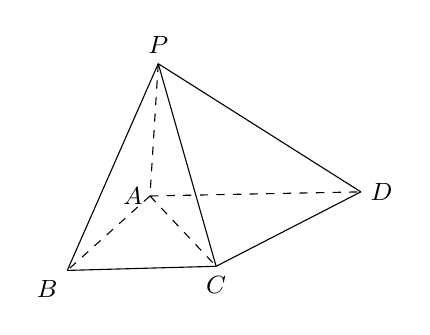
\begin{tikzpicture}[scale=1.05, font=\small]
  \coordinate (P) at (1.45,2.5);
  \coordinate (A) at (1.35,0.9);
  \coordinate (B) at (0.35,0);
  \coordinate (C) at (2.15,0.05);
  \coordinate (D) at (3.9,0.95);
  \draw (P) -- (B)  (P) -- (C)  (P) -- (D);
  \draw (B) -- (C) -- (D);
  \draw[dashed] (P) -- (A);
  \draw[dashed] (A) -- (B)  (A) -- (D)  (A) -- (C);
  \node[above] at (P) {$P$};
  \node[left, inner sep=2.5pt] at (A) {$A$};
  \node[below left] at (B) {$B$};
  \node[below] at (C) {$C$};
  \node[right] at (D) {$D$};
\end{tikzpicture}
\end{center}

  (1) 证明：平面 $PAB\perp$ 平面 $PAD$；

  (2) 设 $PA=AB=\sqrt2$，$BC=2$，$AD=1+\sqrt3$，且点 $P$，$B$，$C$，$D$ 均在球 $O$ 的球面上．

  　① 证明：点 $O$ 在平面 $ABCD$ 内；

  　② 求直线 $AC$ 与 $PO$ 所成角的余弦值．

\end{question}
\begin{question}
\gkti{18}\textbf{（17 分）} 已知椭圆 $C:\dfrac{x^2}{a^2}+\dfrac{y^2}{b^2}=1\ (a>b>0)$ 的离心率为 $\dfrac{2\sqrt2}{3}$，下顶点为 $A$，右顶点为 $B$，$|AB|=\sqrt{10}$．

  (1) 求 $C$ 的方程；

  (2) 已知动点 $P$ 不在 $y$ 轴上，点 $R$ 在射线 $AP$ 上，且满足 $|AP|\cdot|AR|=3$．

  　① 设 $P(m,n)$，求 $R$ 的坐标（用 $m$，$n$ 表示）；

  　② 设 $O$ 为坐标原点，$Q$ 是 $C$ 上的动点，直线 $OR$ 的斜率是直线 $OP$ 的斜率的 $3$ 倍，求 $|PQ|$ 的最大值．

\end{question}
\begin{question}
\gkti{19}\textbf{（17 分）} 

  (1) 求函数 $f(x)=5\cos x-\cos 5x$ 在区间 $\left[0,\dfrac{\pi}{4}\right]$ 的最大值；

  (2) 给定 $\theta\in(0,\pi)$ 和 $a\in\mathbf{R}$，证明：存在 $y\in[a-\theta,\ a+\theta]$ 使得 $\cos y\le\cos\theta$；

  (3) 设 $b\in\mathbf{R}$，若存在 $\varphi\in\mathbf{R}$ 使得 $5\cos x-\cos(5x+\varphi)\le b$ 对 $x\in\mathbf{R}$ 恒成立，求 $b$ 的最小值．

\par\medskip


\end{question}